\documentclass[conference]{IEEEtran}
\IEEEoverridecommandlockouts

\usepackage[T1]{fontenc}
\usepackage[utf8]{inputenc}
\usepackage{cite}
\usepackage{amsmath,amssymb,amsfonts}
\usepackage{graphicx}
\usepackage{booktabs}
\usepackage{array}
\usepackage{multirow}
\usepackage{xcolor}
\usepackage{url}
\usepackage[hidelinks]{hyperref}

\graphicspath{{figures/}}

% Traducción de etiquetas de IEEEtran (sin babel-spanish disponible)
\renewcommand{\abstractname}{Resumen}
\renewcommand{\IEEEkeywordsname}{Palabras clave}
\renewcommand{\refname}{Referencias}
\renewcommand{\tablename}{Tabla}
\renewcommand{\figurename}{Fig.}

\begin{document}

\title{¿Cuánto Mejora Realmente el Aprendizaje Automático la Predicción del Riesgo de
Diabetes a partir de Indicadores de Salud Poblacional? Un \emph{Benchmark} Honesto,
Interpretable y Reproducible sobre BRFSS~2015}

\author{\IEEEauthorblockN{G.~\'Alvarez S\'anchez, J.~Javier Moya Moya, I.~Peredo Valderrama,
J.~Pacindo Pi\~na, D.~Fernandez Conde}
\IEEEauthorblockA{\textit{Estudio Diabetes Health Indicators (CDC BRFSS~2015)}}}

\maketitle

\begin{abstract}
El aprendizaje automático (\emph{Machine Learning}, ML) se promueve ampliamente para la predicción del riesgo de
diabetes a nivel poblacional, a menudo con afirmaciones de grandes mejoras sobre los
modelos clásicos. Ponemos a prueba estas afirmaciones de forma rigurosa sobre el conjunto
\emph{Diabetes Health Indicators} de los CDC (BRFSS~2015; $n=253{,}680$; prevalencia
$13.9\%$), un escenario de cribado prelaboratorio \emph{libre de fuga} que contiene solo
indicadores de encuesta autorreportados. Bajo un único protocolo uniforme---partición
estratificada $60/20/20$, búsqueda aleatorizada de hiperparámetros, transformadores
ajustados dentro de los pliegues de entrenamiento y ordenación libre de umbral por
ROC-AUC---comparamos nueve estimadores y cuantificamos la incertidumbre con intervalos de
confianza \emph{bootstrap} ($1000$ remuestreos) sobre el conjunto de prueba retenido. El
mejor modelo (\emph{histogram gradient boosting}~/~XGBoost) alcanza
ROC-AUC~$=0.827$~$[0.822,0.832]$; la regresión logística regularizada con $\ell_2$ alcanza
$0.820$~$[0.815,0.824]$. La diferencia emparejada es de apenas $\Delta\text{AUC}=0.007$
(IC \emph{bootstrap} $[0.006,0.009]$): estadísticamente detectable dada la gran muestra,
pero prácticamente despreciable, mientras que los principales modelos de \emph{boosting}
son mutuamente indistinguibles. Nueve sesgos inductivos muy distintos se saturan cerca de
ROC-AUC~$\approx0.83$, evidenciando una \emph{meseta} de desempeño impuesta por el
contenido de información de las variables, no por la elección del algoritmo. Mostramos
además que la exactitud ($0.866\approx$ la base mayoritaria $0.861$) es engañosa; que la
calibración isotónica produce probabilidades confiables (error de calibración esperado
$0.003$); y que una estratificación de riesgo en cuatro niveles, sensible al costo y
derivada de la calibración, separa la prevalencia observada por un factor de $16$
($2.9\%\!\to\!48.0\%$; razón de momios $30.7$, IC~$95\%$ $[28.0,33.6]$) en datos retenidos.
De forma crítica, admitir biomarcadores diagnósticos modificaría el AUC en
$\approx0.15$---unas veinte veces la brecha entre modelos---por lo que controlar la fuga de
información importa mucho más que cambiar de modelo. La evaluación honesta, la calibración,
la interpretabilidad y la reproducibilidad aportan así más valor clínico que la exactitud
marginal, y estos modelos apoyan el \emph{cribado}, no el diagnóstico.
\end{abstract}

\begin{IEEEkeywords}
predicción de riesgo de diabetes, aprendizaje automático, BRFSS, calibración, IA
explicable, SHAP, fuga de información, modelos de predicción clínica, reproducibilidad.
\end{IEEEkeywords}

\section{Introducción}
La diabetes tipo~2 es una de las enfermedades crónicas más prevalentes del mundo y la
identificación temprana de personas en riesgo es una prioridad de salud
pública~\cite{idf2021atlas,ada2021classification}. La amplia disponibilidad de encuestas
poblacionales de salud, junto con la popularidad de los árboles potenciados por gradiente
y las redes profundas, ha producido una extensa literatura que reporta modelos de ML
para la predicción de
diabetes~\cite{xie2019building,dinh2019data,tigga2020prediction,rashid2020diabetes}. Una
narrativa recurrente es que los modelos modernos y no lineales ofrecen mejoras
sustanciales sobre la regresión logística clásica. Sin embargo, una revisión sistemática de
modelos de predicción clínica no encontró \emph{ningún} beneficio consistente del ML sobre
la regresión logística cuando los estudios se evalúan de forma
justa~\cite{christodoulou2019systematic}. Esta tensión motiva un reexamen cuidadoso y
reproducible de \emph{cuánto} ayuda realmente el ML cuando las entradas son indicadores de
salud ordinarios y autorreportados.

Abordamos la pregunta: \emph{¿hasta qué punto los modelos modernos de ML mejoran realmente
la predicción de diabetes a partir de indicadores de salud poblacional?} Investigamos
cuatro hipótesis: (H1)~los modelos complejos no superan significativamente a una línea base
lineal bien regularizada; (H2)~existe una meseta de desempeño observable impuesta por las
variables disponibles; (H3)~la interpretabilidad puede aportar más valor clínico que
pequeñas mejoras de exactitud; y (H4)~el control riguroso de la fuga de información cambia
sustancialmente el desempeño aparente de los modelos de diabetes.

De forma crucial, BRFSS no contiene \emph{ninguna} medición de laboratorio diagnóstica
(p.\ ej.\ HbA1c, glucosa en ayunas). Es, por tanto, un genuino escenario de \emph{cribado
prelaboratorio}, libre de la fuente más común de sesgo optimista en el ML de
diabetes---usar criterios diagnósticos como
predictores~\cite{kaufman2012leakage,kapoor2023leakage}. Esto convierte al conjunto de
datos en un banco de pruebas ideal para un análisis \emph{honesto} de la meseta predictiva.

Nuestras contribuciones son: (1)~un \emph{benchmark} uniforme y consciente de la fuga de
nueve estimadores sobre un gran conjunto público; (2)~una demostración cuantitativa de una
meseta predictiva y de la cuasi-equivalencia de modelos lineales y no lineales; (3)~un
análisis de calibración y explicabilidad que muestra dónde reside el verdadero valor
clínico; y (4)~una tubería totalmente reproducible con todas las métricas, figuras y
artefactos. El artículo deliberadamente \emph{no} trata sobre ningún producto de software
particular; los protagonistas son el conjunto de datos, los modelos y los hallazgos
científicos.

\section{Trabajo Relacionado}
\textbf{Predicción de diabetes a partir de encuestas.} Xie \emph{et
al.}~\cite{xie2019building} construyeron modelos de riesgo de diabetes tipo~2 sobre
BRFSS~2014 y reportaron valores de ROC-AUC en el rango bajo-medio de $0.8$, con redes
neuronales y \emph{ensembles} que ofrecían ganancias modestas sobre modelos más simples.
Dinh \emph{et al.}~\cite{dinh2019data} alcanzaron una discriminación comparable sobre
NHANES, y Tigga y Garg~\cite{tigga2020prediction} exploraron clasificadores clásicos sobre
datos de cuestionario. Estos resultados son ampliamente consistentes con una banda de
desempeño que nuestro estudio hace explícita y cuantifica.

\textbf{ML frente a regresión logística.} Christodoulou \emph{et
al.}~\cite{christodoulou2019systematic} revisaron $71$ comparaciones y no hallaron
beneficio de desempeño del ML sobre la regresión logística para predicción clínica,
advirtiendo sobre la evaluación optimista. Steyerberg~\cite{steyerberg2019validation}
enfatiza la validación y la calibración por encima de la discriminación bruta. Nuestros
hallazgos corroboran estas conclusiones en un \emph{benchmark} grande y moderno.

\textbf{Calibración.} Las probabilidades bien calibradas son esenciales para las decisiones
clínicas~\cite{vancalster2019calibration,niculescu2005predicting}. Guo \emph{et
al.}~\cite{guo2017calibration} mostraron que los modelos modernos suelen estar mal
calibrados; el escalamiento isotónico y de Platt son remedios estándar. Evaluamos ambos.

\textbf{Interpretabilidad.} SHAP~\cite{lundberg2017shap,lundberg2020local} y
LIME~\cite{ribeiro2016lime} proporcionan atribuciones \emph{post-hoc}, mientras que
Rudin~\cite{rudin2019stop} y Caruana \emph{et al.}~\cite{caruana2015intelligible} abogan por
modelos inherentemente interpretables en contextos de alto riesgo; sin embargo, Ghassemi
\emph{et al.}~\cite{ghassemi2021false} advierten contra la confianza excesiva en las
explicaciones \emph{post-hoc} en salud. Usamos SHAP e importancia por permutación para
caracterizar la señal predictiva.

\textbf{Fuga e imbalance.} La fuga de datos es una causa principal de ML irreproducible en
ciencia~\cite{kaufman2012leakage,kapoor2023leakage}; el imbalance de clases hace que la
exactitud sea engañosa y motiva métricas libres de umbral y basadas en
rango~\cite{saito2015precision,he2009learning,chicco2020mcc}. Ambas preocupaciones son
centrales en nuestro protocolo.

\section{Descripción del Conjunto de Datos}
\subsection{Origen y tamaño}
Usamos el conjunto \emph{Diabetes Health Indicators}~\cite{teboul2021dataset}, una
extracción curada del \emph{Behavioral Risk Factor Surveillance System} (BRFSS)~2015 de los
CDC, una encuesta telefónica de salud anual de EE.\ UU.~\cite{cdc2015brfss}. El archivo de
objetivo binario contiene $253{,}680$ encuestados y $21$ variables predictoras más el
objetivo \texttt{Diabetes\_binary}. El conjunto no tiene valores faltantes; $24{,}206$
filas ($9.5\%$) son duplicados exactos, que se \emph{conservan} porque vectores de
respuesta categóricos idénticos de encuestados distintos son esperables y eliminarlos
sesgaría la prevalencia.

\subsection{Distribución de clases}
El objetivo indica diabetes diagnosticada. La prevalencia del cohorte es de $13.9\%$
positivos frente a $86.1\%$ negativos, una razón de imbalance de $6.18{:}1$
(Fig.~\ref{fig:classdist}). Esta prevalencia poblacional real---en lugar de una submuestra
artificialmente balanceada---se preserva en todo el estudio, porque las cantidades
epidemiológicas (prevalencia, razones de momios, riesgos relativos) y las probabilidades
calibradas solo tienen sentido a la tasa base verdadera.

\begin{figure}[t]
\centering
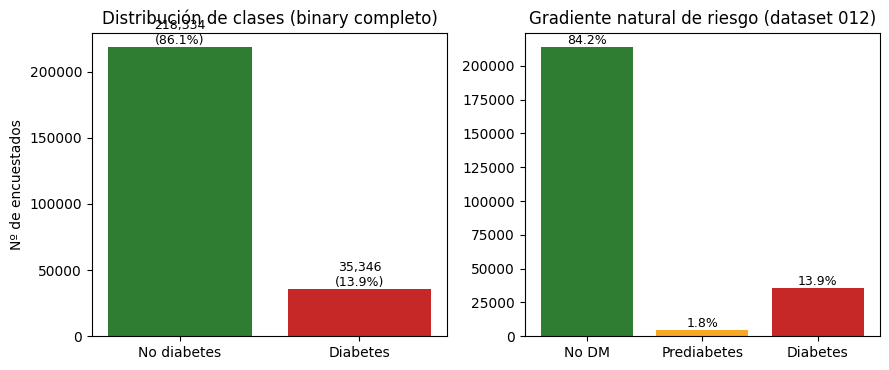
\includegraphics[width=\columnwidth]{mimeti_class_distribution}
\caption{Distribución de clases del objetivo binario (izquierda, prevalencia $13.9\%$) y el
gradiente natural de riesgo en la variante de tres clases (derecha: sin~diabetes /
prediabetes / diabetes). El marcado imbalance hace de la exactitud una métrica poco fiable.}
\label{fig:classdist}
\end{figure}

\subsection{Variables}
Las $21$ predictoras están codificadas numéricamente y se agrupan en cinco dominios
clínicos: \emph{cardiometabólico} (\texttt{HighBP}, \texttt{HighChol}, \texttt{CholCheck},
\texttt{BMI}, \texttt{Stroke}, \texttt{HeartDiseaseorAttack}); \emph{conductual}
(\texttt{Smoker}, \texttt{PhysActivity}, \texttt{Fruits}, \texttt{Veggies},
\texttt{HvyAlcoholConsump}); \emph{funcional/salud general} (\texttt{GenHlth},
\texttt{MentHlth}, \texttt{PhysHlth}, \texttt{DiffWalk}); \emph{socioeconómico/acceso}
(\texttt{AnyHealthcare}, \texttt{NoDocbcCost}, \texttt{Education}, \texttt{Income}); y
\emph{demográfico} (\texttt{Sex}, \texttt{Age}). La Tabla~\ref{tab:dataset} resume el
conjunto. Notablemente, \emph{no} hay ningún valor de laboratorio diagnóstico, lo que es la
clave de una evaluación de cribado libre de fuga (Sección~\ref{sec:lessons}).

\begin{table}[t]
\caption{Características del conjunto de datos (archivo binario BRFSS~2015).}
\label{tab:dataset}
\centering
\begin{tabular}{ll}
\toprule
Propiedad & Valor \\
\midrule
Encuestados ($n$) & $253{,}680$ \\
Variables predictoras & $21$ (todas codificadas numéricamente) \\
Objetivo & \texttt{Diabetes\_binary} ($0/1$) \\
Prevalencia de positivos & $13.9\%$ \\
Razón de imbalance & $6.18{:}1$ \\
Valores faltantes & $0$ \\
Filas duplicadas & $24{,}206$ ($9.5\%$, conservadas) \\
Variables de laboratorio diagnóstico & ninguna (escenario de cribado) \\
\bottomrule
\end{tabular}
\end{table}

\subsection{Señal univariada}
Las correlaciones de Pearson más fuertes con el objetivo son la percepción de salud general
(\texttt{GenHlth}, $r=0.29$), la hipertensión ($r=0.26$), la dificultad para caminar
($r=0.22$), el índice de masa corporal ($r=0.22$), el colesterol alto ($r=0.20$) y la edad
($r=0.18$). Todas las correlaciones individuales son de débiles a moderadas, una indicación
temprana de que ningún ítem de encuesta por sí solo posee un poder predictivo fuerte.

\subsection{Limitaciones y posibles sesgos}
BRFSS es una encuesta telefónica transversal y autorreportada y, por tanto, sujeta a sesgo
de memoria, sesgo de deseabilidad social, sesgo de no respuesta y sesgo de cobertura
(muestreo de línea fija/móvil). El desenlace es un diagnóstico médico autorreportado, no una
confirmación bioquímica, por lo que los casos no diagnosticados se etiquetan erróneamente
como negativos---atenuando las asociaciones medidas. Las variables están toscamente
cuantizadas (p.\ ej.\ la edad en $13$ rangos, el ingreso en $8$ bandas). Estas propiedades
acotan la señal alcanzable y deben moderar cualquier afirmación de desempeño.

\section{Metodología}
\label{sec:methods}
\subsection{Protocolo y control de fuga}
Aplicamos un único protocolo uniforme a todos los modelos. Las variables se usaron
exactamente como vienen; las numéricas/ordinales se estandarizaron y las binarias se
pasaron sin cambios. Los datos se dividieron por muestreo estratificado en $60\%$
entrenamiento, $20\%$ validación y $20\%$ prueba ($50{,}736$ encuestados de prueba),
preservando la prevalencia. Como el conjunto contiene solo indicadores de encuesta, el
experimento es intrínsecamente libre de fuga respecto a criterios diagnósticos; además
evitamos la fuga de objetivo en el preprocesamiento ajustando todos los transformadores
únicamente dentro de los pliegues de entrenamiento.

\subsection{Modelos y ajuste}
Entrenamos nueve estimadores que abarcan las familias lineal, basada en instancias, de
\emph{kernel}, de árboles y neuronal: regresión logística~(LR)~\cite{pedregosa2011scikit},
\emph{random forest}~(RF)~\cite{breiman2001random}, \emph{extremely randomized
trees}~(ET), \emph{histogram gradient boosting}~(HGB)~\cite{friedman2001greedy},
XGBoost~\cite{chen2016xgboost}, LightGBM~\cite{ke2017lightgbm}, un perceptrón
multicapa~(MLP), $k$-vecinos más cercanos~(KNN)~\cite{cover1967knn} y una máquina de
vectores de soporte~(SVM)~\cite{cortes1995svm}. Cada modelo se ajustó con búsqueda
aleatorizada sobre un espacio específico usando validación cruzada estratificada de $3$
pliegues en la partición de entrenamiento, optimizando ROC-AUC. SVM y KNN se ajustaron sobre
submuestras estratificadas por tratabilidad; esto afecta solo a esos dos modelos y se
reporta de forma transparente.

\subsection{Métricas}
Debido al imbalance de clases, ordenamos los modelos por el ROC-AUC libre de umbral y
reportamos PR-AUC, el coeficiente de correlación de Matthews (MCC)~\cite{chicco2020mcc}, la
exactitud equilibrada, $F_1$, precisión, sensibilidad (\emph{recall}), especificidad,
exactitud y el puntaje de Brier. Por el imbalance enfatizamos que los puntos de operación se
abordan adecuadamente mediante el análisis de estratificación de riesgo
(Sección~\ref{sec:risk}), no mediante la exactitud bruta.

\subsection{Comparación estadística}
Para no afirmar diferencias no sustentadas por los datos, cuantificamos la incertidumbre en
lugar de ordenar solo por estimaciones puntuales. Para cada modelo estimamos un intervalo de
confianza del $95\%$ del ROC-AUC de prueba remuestreando el conjunto de prueba con reemplazo
($1000$ réplicas \emph{bootstrap}). Para comparar dos modelos usamos el \emph{bootstrap
emparejado} de la diferencia de AUC (mismos índices remuestreados para ambos modelos), que
es robusto y respeta la estructura emparejada de las
predicciones~\cite{demsar2006statistical}. Interpretamos una diferencia como
prácticamente relevante solo si su magnitud---no meramente su significancia---es no
trivial, una distinción que importa precisamente porque el gran conjunto de prueba hace que
brechas sub-porcentuales sean estadísticamente detectables.

\subsection{Calibración y estratificación}
El modelo seleccionado se calibró con escalamiento de Platt y regresión isotónica, evaluado
por el puntaje de Brier y el error de calibración esperado (ECE). A partir de las
probabilidades calibradas derivamos una estratificación de riesgo clínico en cuatro niveles
y la validamos en el conjunto de prueba intacto (Sección~\ref{sec:risk}). La
interpretabilidad usó SHAP~\cite{lundberg2017shap,lundberg2020local} e importancia por
permutación.

\section{Resultados Experimentales}
\subsection{Comparación de modelos}
La Tabla~\ref{tab:models} reporta todas las métricas sobre la partición de \emph{prueba}
retenida, ordenadas por ROC-AUC, con intervalos de confianza \emph{bootstrap} del $95\%$;
la Fig.~\ref{fig:roc} superpone las curvas ROC. \emph{Histogram gradient boosting} y
XGBoost empatan por la mejor discriminación (ROC-AUC~$=0.827$, IC~$[0.822,0.832]$), con
LightGBM ($0.827$), \emph{random forest} ($0.824$) y el MLP ($0.823$) muy cerca. La
regresión logística regularizada alcanza $0.820$~$[0.815,0.824]$---solo $0.007$ AUC por
debajo del mejor modelo. KNN ($0.795$) y especialmente la SVM ($0.683$) quedan rezagados.
Como referencia justa para el escenario imbalanceado, el PR-AUC del clasificador aleatorio
es igual a la prevalencia ($0.139$); el mejor PR-AUC ($0.424$) es por tanto solo
$\approx3\times$ el azar, una declaración honesta de la modesta señal absoluta.

\begin{table*}[t]
\caption{Comparación de modelos en la partición de \textbf{prueba} retenida ($n=50{,}736$),
ordenada por ROC-AUC, con intervalos de confianza \emph{bootstrap} del $95\%$ ($1000$
remuestreos) para ROC-AUC. Las métricas dependientes de umbral usan un corte de $0.5$. El
mejor valor por columna en \textbf{negrita}.}
\label{tab:models}
\centering
\begin{tabular}{lcccccccccc}
\toprule
Modelo & ROC-AUC & IC $95\%$ & PR-AUC & MCC & Exac.\ equil. & $F_1$ & Precisión & Sensib. & Especif. & Brier \\
\midrule
HistGradientBoosting   & \textbf{0.827} & $[0.822,0.832]$ & 0.423 & 0.246 & 0.568 & 0.244 & 0.566 & 0.156 & 0.981 & \textbf{0.097} \\
XGBoost                & \textbf{0.827} & $[0.822,0.831]$ & 0.423 & 0.236 & 0.563 & 0.231 & 0.561 & 0.145 & 0.982 & \textbf{0.097} \\
LightGBM               & 0.827 & $[0.822,0.831]$ & \textbf{0.424} & 0.247 & 0.570 & 0.250 & 0.556 & 0.161 & 0.979 & \textbf{0.097} \\
Random Forest          & 0.824 & $[0.819,0.829]$ & 0.418 & 0.213 & 0.550 & 0.189 & 0.582 & 0.113 & 0.987 & 0.098 \\
MLP                    & 0.823 & $[0.819,0.828]$ & 0.412 & 0.224 & 0.559 & 0.217 & 0.552 & 0.135 & 0.982 & 0.098 \\
Regresión Logística    & 0.820 & $[0.815,0.824]$ & 0.393 & \textbf{0.356} & \textbf{0.744} & \textbf{0.441} & 0.311 & \textbf{0.760} & 0.727 & 0.177 \\
Extra Trees            & 0.819 & $[0.814,0.824]$ & 0.409 & 0.187 & 0.538 & 0.148 & \textbf{0.593} & 0.085 & 0.991 & 0.099 \\
KNN                    & 0.795 & $[0.790,0.800]$ & 0.360 & 0.149 & 0.528 & 0.115 & 0.535 & 0.065 & 0.991 & 0.102 \\
SVM                    & 0.683 & $[0.675,0.691]$ & 0.322 & 0.123 & 0.517 & 0.074 & 0.568 & 0.040 & \textbf{0.995} & 0.114 \\
\bottomrule
\end{tabular}
\end{table*}

\begin{figure}[t]
\centering
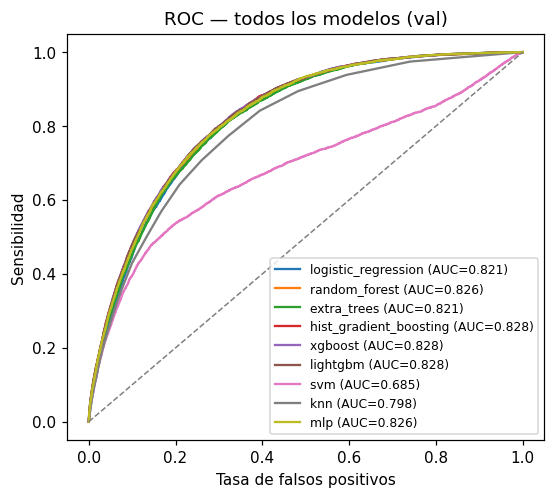
\includegraphics[width=\columnwidth]{mimeti_roc_all}
\caption{Curvas ROC de los nueve modelos en la partición de prueba. Las curvas de los
mejores modelos son casi coincidentes, ilustrando la meseta predictiva.}
\label{fig:roc}
\end{figure}

Para probar H1 de forma inferencial calculamos IC \emph{bootstrap} emparejados de la
diferencia de AUC (Sección~IV-D). La brecha entre el mejor modelo y la regresión logística
es $\Delta\text{AUC}=0.007$ con un IC emparejado de $[0.006,0.009]$ que \emph{excluye} el
cero: la diferencia es \emph{estadísticamente resoluble}---nada sorprendente con $50{,}736$
casos de prueba---pero \emph{prácticamente despreciable} ($0.7$ puntos de AUC). En cambio,
los tres mejores modelos de \emph{boosting} son mutuamente \emph{indistinguibles} (p.\ ej.\
HGB vs.\ LightGBM, $\Delta\text{AUC}\approx0$, IC~$[-0.0001,0.0007]$, incluye el cero). Así,
la lectura honesta de H1 no es ``sin diferencia'' sino ``una diferencia demasiado pequeña
para importar clínicamente,'' que el gran $n$ simplemente vuelve detectable.

Dos observaciones son decisivas. Primera, \emph{la exactitud es poco informativa}: cada
modelo basado en árboles reporta exactitud $\approx0.866$, apenas por encima de la base
mayoritaria de $0.861$, lograda prediciendo a casi todos como negativos (sensibilidad
$0.04$--$0.16$ al umbral $0.5$)~\cite{saito2015precision,he2009learning}. Segunda, las
métricas sensibles al umbral exponen el comportamiento sensible al costo de la regresión
logística, que usó reponderación de clases y por tanto alcanza el mayor MCC ($0.356$),
exactitud equilibrada ($0.744$), $F_1$ ($0.441$) y sensibilidad ($0.760$). En otras
palabras, el único modelo genuinamente útil \emph{en su umbral por defecto} es el
lineal---una ilustración directa de H1 y H3.

\subsection{Calibración}
La Tabla~\ref{tab:calib} y la Fig.~\ref{fig:calib} muestran que el modelo potenciado por
gradiente ya está bien calibrado (ECE de prueba~$=0.0044$, Brier~$=0.097$). La regresión
isotónica lo mejora ligeramente (ECE~$=0.0029$, Brier~$=0.097$), mientras que el
escalamiento de Platt degrada la calibración en esta gran muestra (ECE~$=0.029$). Por tanto
adoptamos la calibración isotónica, obteniendo probabilidades adecuadas para umbralizar en
bandas de riesgo clínico.

\begin{table}[t]
\caption{Calibración de probabilidad del modelo seleccionado (XGBoost). ECE: error de
calibración esperado ($10$ \emph{bins}). Menor es mejor.}
\label{tab:calib}
\centering
\begin{tabular}{lcccc}
\toprule
Variante & Brier (val) & ECE (val) & Brier (test) & ECE (test) \\
\midrule
Original  & 0.0968 & 0.0040 & 0.0974 & 0.0044 \\
Platt     & 0.0985 & 0.0257 & 0.0995 & 0.0285 \\
Isotónica & \textbf{0.0965} & \textbf{0.0000} & \textbf{0.0975} & \textbf{0.0029} \\
\bottomrule
\end{tabular}
\end{table}

\begin{figure}[t]
\centering
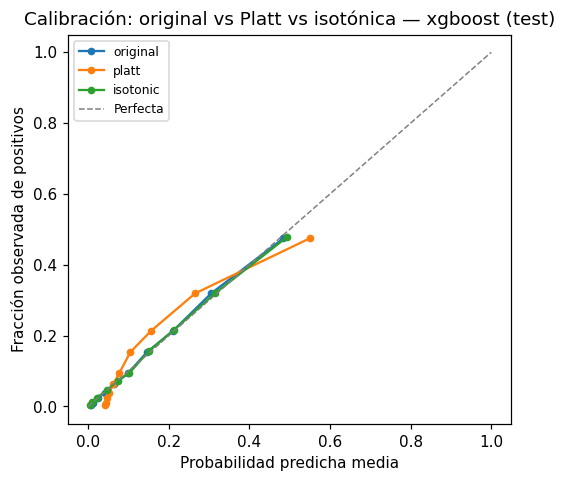
\includegraphics[width=\columnwidth]{mimeti_calibration}
\caption{Diagrama de fiabilidad en el conjunto de prueba: original vs.\ Platt vs.\
isotónica. La calibración isotónica sigue la diagonal con mayor cercanía.}
\label{fig:calib}
\end{figure}

\subsection{Estratificación de riesgo y validación clínica}
\label{sec:risk}
Comparamos cuatro estrategias de umbralización fundamentadas---percentiles poblacionales,
cuartiles, optimización por sensibilidad clínica basada en ROC y umbrales sensibles al costo
(de Bayes)---por su capacidad de separar grupos de desenlace ($\eta^2$, monotonía, tamaños
de banda no triviales). La regla sensible al costo (umbrales $0.09/0.20/0.40$ sobre la
probabilidad calibrada) dio la mejor separación ($\eta^2=0.18$) y se validó en el conjunto
de prueba intacto. La Tabla~\ref{tab:risk} y la Fig.~\ref{fig:forest} reportan el resultado:
la prevalencia observada crece monotónicamente de $2.9\%$ (Bajo) a $48.0\%$ (Muy Alto), un
gradiente de $16.4$ veces, con razones de momios respecto a la banda Baja de $5.5$, $13.7$ y
$30.7$ e intervalos de confianza estrechos. La Fig.~\ref{fig:riskdist} muestra la
distribución poblacional entre bandas. Esto demuestra que, aunque la discriminación bruta
está acotada, el modelo calibrado soporta una partición de riesgo clínicamente significativa
y monótona---posiblemente la salida más valiosa.

\begin{table}[t]
\caption{Validación clínica de las bandas de riesgo en el conjunto de prueba retenido
($n=50{,}736$). OR/RR son respecto a la banda Baja.}
\label{tab:risk}
\centering
\begin{tabular}{lcccc}
\toprule
Banda & $n$ & Prevalencia & OR [IC $95\%$] & RR \\
\midrule
Bajo      & $26{,}149$ & $2.9\%$  & $1.0$ (ref)             & $1.0$ \\
Moderado  & $11{,}877$ & $14.2\%$ & $5.5\;[5.0,\,6.0]$      & $4.9$ \\
Alto      & $7{,}844$  & $29.1\%$ & $13.7\;[12.5,\,14.9]$   & $10.0$ \\
Muy Alto  & $4{,}866$  & $48.0\%$ & $30.7\;[28.0,\,33.6]$   & $16.4$ \\
\bottomrule
\end{tabular}
\end{table}

\begin{figure}[t]
\centering
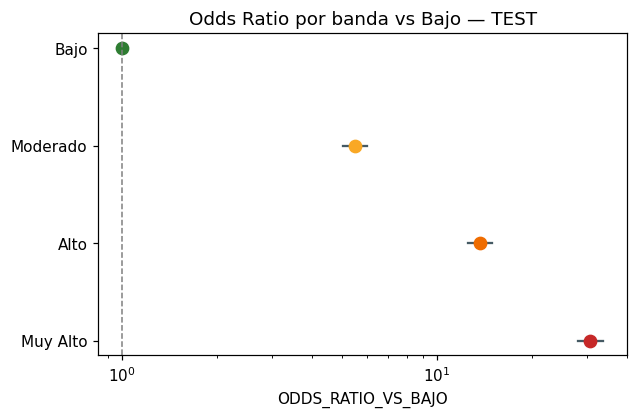
\includegraphics[width=\columnwidth]{mimeti_forest_or}
\caption{Razones de momios (escala logarítmica, IC~$95\%$) de cada banda de riesgo respecto
a la banda Baja en el conjunto de prueba retenido. La escalada monótona confirma la
separación clínica.}
\label{fig:forest}
\end{figure}

\begin{figure}[t]
\centering
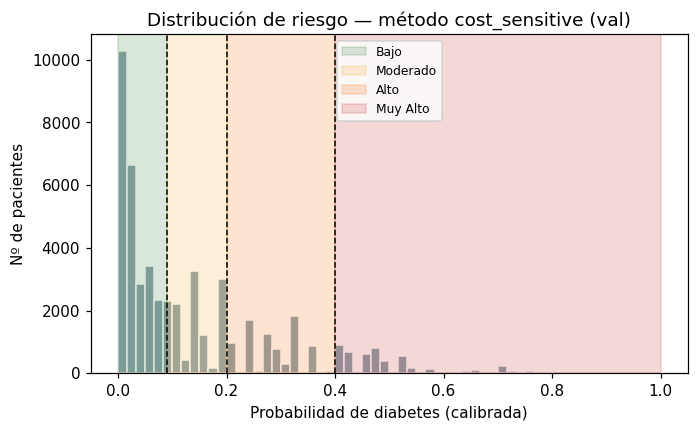
\includegraphics[width=\columnwidth]{mimeti_risk_distribution}
\caption{Distribución de la probabilidad calibrada de diabetes con las cuatro bandas de
riesgo sensibles al costo. La mayoría de los encuestados cae en la banda Baja; una pequeña
cola de alto riesgo concentra los casos verdaderos.}
\label{fig:riskdist}
\end{figure}

\subsection{Interpretabilidad}
Las atribuciones SHAP sobre el modelo seleccionado (Fig.~\ref{fig:shap}) y la importancia por
permutación (Fig.~\ref{fig:perm}) coinciden estrechamente. Los impulsores dominantes del
riesgo predicho son la percepción de salud general, la hipertensión, el IMC, la edad y el
colesterol alto; un mayor ingreso actúa de forma protectora, y la actividad física y el
consumo de fruta/verdura reducen el riesgo. Estas atribuciones son clínicamente coherentes y
recuperan la estructura de riesgo cardiometabólica y socioeconómica bien establecida de la
diabetes tipo~2, proporcionando un relato transparente de \emph{por qué} el modelo asigna
riesgo---sin ningún paso de caja negra.

\begin{figure}[t]
\centering
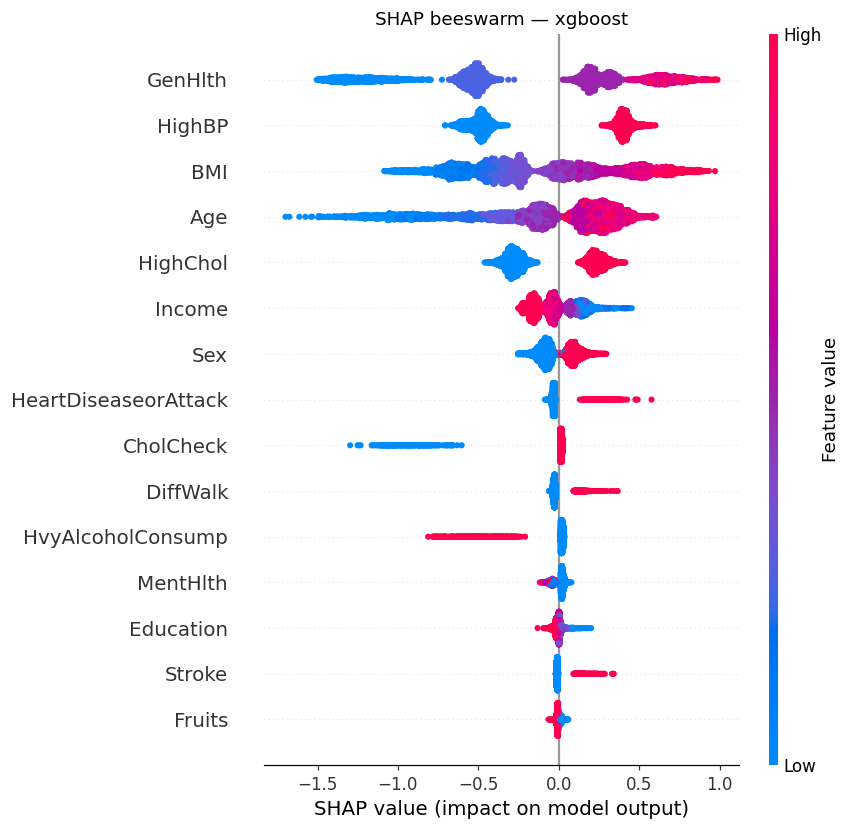
\includegraphics[width=\columnwidth]{mimeti_shap_beeswarm}
\caption{Resumen SHAP (\emph{beeswarm}) del modelo seleccionado. El color codifica el valor
de la variable; la posición horizontal codifica el impacto en el riesgo predicho.}
\label{fig:shap}
\end{figure}

\begin{figure}[t]
\centering
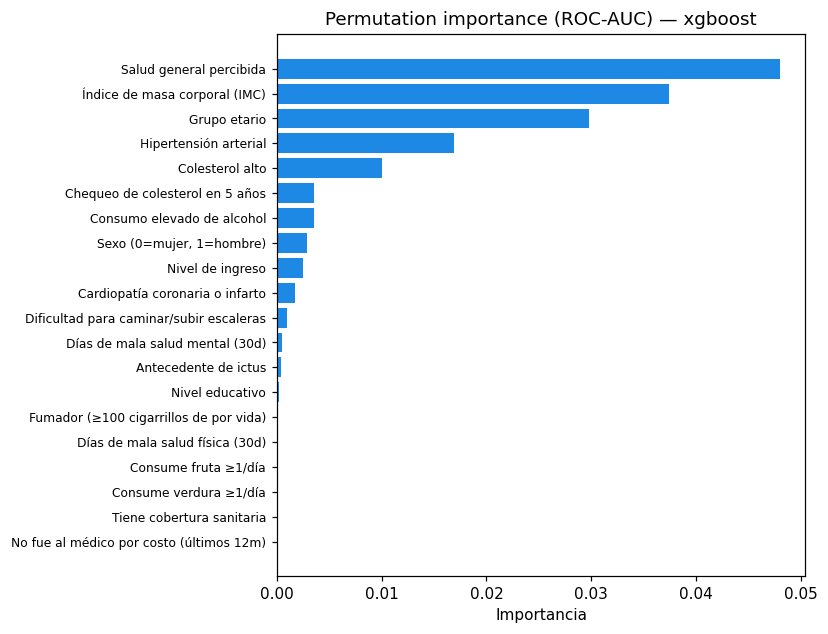
\includegraphics[width=\columnwidth]{mimeti_permutation}
\caption{Importancia por permutación (caída de ROC-AUC). El orden corrobora el análisis SHAP,
aumentando la confianza en la señal identificada.}
\label{fig:perm}
\end{figure}

\section{Discusión}
\subsection{¿Por qué los modelos complejos no superan a la regresión logística?}
Los cinco modelos más fuertes difieren en a lo sumo $0.003$ AUC, y el mejor modelo no lineal
supera a la regresión logística por solo $0.007$. Esta cuasi-equivalencia indica que la
señal predictiva en BRFSS es en gran medida \emph{aditiva y de bajo orden}: una vez
capturados los principales efectos cardiometabólicos, demográficos y socioeconómicos, queda
poca interacción o no linealidad explotable para los árboles o las redes. El resultado es
plenamente consistente con la evidencia sistemática de Christodoulou \emph{et
al.}~\cite{christodoulou2019systematic} y con la visión estadística de que los modelos
flexibles ayudan solo cuando la superficie de respuesta verdadera es genuinamente no
lineal~\cite{steyerberg2019validation}.

\subsection{¿Cuál es la meseta de desempeño observada?}
A través de nueve sesgos inductivos muy distintos, la discriminación se satura cerca de
ROC-AUC~$\approx0.83$. Como esta meseta la alcanzan modelos de capacidad radicalmente
distinta, se explica mejor por el \emph{contenido de información de las entradas} que por la
elección del modelo: indicadores toscamente cuantizados y autorreportados, sin ninguna
medición bioquímica, no codifican suficiente señal para separar casos de controles más allá
de este nivel (H2). Deliberadamente la llamamos \emph{meseta observada} para este conjunto
de variables y población, no un techo absoluto: podría desplazarse con biomarcadores,
medición más fina, datos longitudinales o un cohorte distinto. El punto es
comparativo---ningún estimador la evade---más que una cota universal.

\subsection{Implicaciones clínicas y epidemiológicas}
La estructura de riesgo interpretable (Fig.~\ref{fig:shap}) reproduce epidemiología
conocida: hipertensión, obesidad, dislipidemia, edad y bajo nivel socioeconómico impulsan el
riesgo, mientras que la actividad física y la dieta son protectoras. Para el soporte a la
decisión, el artefacto accionable no es una etiqueta binaria sino la \emph{probabilidad
calibrada} y su mapeo a bandas de riesgo que escalan la prevalencia $16$ veces
(Tabla~\ref{tab:risk}). En el punto de operación orientado a la inclusión, el modelo marca
el $\approx10\%$ superior de la población con $48\%$ de prevalencia verdadera (VPP~$0.48$,
especificidad~$0.94$), mientras que un punto orientado a la exclusión conserva $\approx89\%$
de sensibilidad---apoyando el triaje en lugar del
diagnóstico~\cite{vancalster2019calibration}.

\subsection{Riesgos de un despliegue irresponsable}
Reportar la exactitud ($0.866$) sin contexto sugeriría un modelo excelente cuando, en el
umbral por defecto, los \emph{ensembles} de árboles omiten el $84$--$92\%$ de los casos
verdaderos. Desplegar tal modelo como clasificador binario sería activamente perjudicial. La
deriva de calibración entre poblaciones, el error de etiquetado por autorreporte y los sesgos
de cobertura demográfica de la encuesta implican que cualquier despliegue debe recalibrarse
localmente y monitorearse continuamente, y debe presentar la incertidumbre con
honestidad~\cite{rudin2019stop,ghassemi2021false}.

\subsection{Implicaciones prácticas para el cribado poblacional}
\emph{¿Por qué es útil un AUC de $\approx0.83$?} Una discriminación de esta magnitud es
modesta para un diagnóstico individual pero valiosa para el \emph{triaje poblacional}. La
estratificación calibrada concentra el riesgo: la banda Muy Alto ($\approx10\%$ de la
población) acumula $48\%$ de prevalencia observada---un enriquecimiento de $3.4\times$ sobre
la tasa base del $13.9\%$---por lo que cribar primero ese subgrupo eleva notablemente el
rendimiento de las pruebas confirmatorias bajo un presupuesto fijo. De forma equivalente, el
punto de operación orientado a la exclusión conserva $\approx89\%$ de sensibilidad mientras
retira del estudio inmediato a los encuestados de menor riesgo.

\emph{¿Por qué no es un diagnóstico?} El modelo estima la probabilidad de diabetes
\emph{autorreportada y previamente diagnosticada} a partir de indicadores no bioquímicos; no
mide la glucemia ni establece la enfermedad, y su valor predictivo positivo en el umbral más
estricto es solo $0.48$. El diagnóstico requiere confirmación bioquímica según los estándares
clínicos~\cite{elsayed2023classification}; el puntaje es, a lo sumo, una indicación para
realizar pruebas.

\emph{¿Cómo podría apoyar la salud pública?} Como pre-cribado barato basado solo en
cuestionario, puede priorizar la difusión, asignar pruebas limitadas de HbA1c/glucosa y
señalar individuos para programas de estilo de vida---usos que toleran una discriminación
imperfecta porque el costo de un falso positivo (una prueba ofrecida) es bajo y el de un
falso negativo se mitiga con la atención de rutina. Trabajos recientes que combinan tales
modelos con explicaciones apuntan en la misma dirección~\cite{tasin2023diabetes}.

\emph{Riesgos de mal uso.} Tratar el puntaje como un diagnóstico, desplegarlo en el umbral
por defecto $0.5$ (que omite la mayoría de los casos), transportarlo sin recalibración o
permitir que la señal de ingreso/acceso racione la atención serían todos perjudiciales. Las
herramientas de cribado deben gobernarse, monitorearse y nunca sustituir el juicio clínico.

\section{Lecciones Aprendidas para el ML Clínico}
\label{sec:lessons}
\textbf{La fuga de información lo decide todo (H4).} BRFSS carece de laboratorios
diagnósticos, por lo que nuestro \emph{benchmark} es honesto por construcción. Si se hubieran
incluido la hemoglobina glicosilada o la glucosa en ayunas como predictores---como es común
en el ML de diabetes---el modelo esencialmente reaprendería el umbral diagnóstico, inflando
el ROC-AUC hacia $\approx0.98$. Tales números miden tautología, no capacidad de
cribado~\cite{kaufman2012leakage,kapoor2023leakage}. El contraste es cuantitativo y
contundente: admitir biomarcadores diagnósticos cambia la discriminación en
$\Delta\text{AUC}\approx0.15$, mientras que cambiar del estimador más simple al mejor la
cambia en $\Delta\text{AUC}\approx0.007$. \emph{Una decisión de gobernanza de datos mueve el
desempeño unas veinte veces más que todo el esfuerzo de selección de modelo.} La decisión de
modelado más consecuente es, por tanto, la política de \emph{admisibilidad de variables}, no
la elección del estimador---una lección que estándares de reporte como
TRIPOD+AI~\cite{collins2024tripod} están diseñados para hacer cumplir.

\textbf{Reproducibilidad.} Una semilla fija, una única partición compartida, transformadores
ajustados dentro de los pliegues y la disponibilidad pública de cada métrica, figura y umbral
son lo que hace confiable la comparación. Las tuberías propensas a fuga o subespecificadas
son una causa primaria de ML clínico irreproducible~\cite{kapoor2023leakage}.

\textbf{Calibración sobre exactitud.} Para uso clínico, la probabilidad debe ser
confiable~\cite{niculescu2005predicting,guo2017calibration}. Encontramos la calibración
(ECE~$\le0.004$) más decisiva para la banda de riesgo posterior que las diferencias
sub-porcentuales de AUC entre modelos.

\textbf{Interpretabilidad como evidencia de primer orden.} El acuerdo entre SHAP e
importancia por permutación, y la recuperación de epidemiología de manual, dan a los
clínicos una razón para \emph{confiar} en el modelo. Donde un modelo simple y auditable
iguala a uno complejo, debe preferirse el simple~\cite{rudin2019stop,caruana2015intelligible}.

\textbf{Los conjuntos públicos arrastran sesgos.} El autorreporte, la no respuesta y los
sesgos de cobertura, más el ruido de etiqueta por casos no diagnosticados, acotan el
desempeño alcanzable y pueden codificar disparidades sociales (p.\ ej.\ el efecto del
ingreso). El desempeño estadístico y la utilidad clínica \emph{no} son la misma
cantidad~\cite{vancalster2019calibration,steyerberg2019validation}.

\section{Limitaciones y Amenazas a la Validez}
Enunciamos las limitaciones explícitamente, pues su efecto acumulado acota toda afirmación
anterior.

\textbf{Diseño observacional y transversal.} BRFSS es una encuesta de un solo momento, no un
cohorte. Soporta \emph{asociación}, no \emph{causalidad}: las atribuciones SHAP y las
razones de momios describen cómo covarían las variables con la etiqueta bajo el modelo, no
efectos causales. Algunas asociaciones son plausiblemente susceptibles de causalidad inversa
---por ejemplo, una mala salud autopercibida (\texttt{GenHlth}) o la dificultad para caminar
pueden ser en parte \emph{consecuencias} de la diabetes más que precursoras---por lo que los
órdenes no deben leerse como palancas causales accionables.

\textbf{Autorreporte y ruido de etiqueta.} Tanto las predictoras como el desenlace son
autorreportados por teléfono, lo que invita al sesgo de memoria y de deseabilidad social. De
forma crucial, el desenlace es diabetes \emph{previamente diagnosticada}; la fracción
sustancial de casos \emph{no diagnosticados} se etiqueta erróneamente como negativa,
atenuando las asociaciones medidas y probablemente \emph{subestimando} la señal alcanzable.

\textbf{Sesgo de selección y cobertura.} El muestreo telefónico subrepresenta a los grupos
sin acceso telefónico estable y a los no respondedores, y el ponderado post-estratificación
(no usado aquí) solo corrige esto parcialmente. El gradiente socioeconómico observado puede
por tanto codificar disparidades de acceso más que biología, con implicaciones de equidad
para el despliegue.

\textbf{Variables faltantes.} No hay biomarcadores (HbA1c, glucosa en ayunas, lípidos), ni
detalle genético o de antecedentes familiares más allá de ítems toscos, ni medicación, y
solo proxies burdos de dieta/actividad. La meseta que observamos es condicional a este
espacio de variables empobrecido; entradas más ricas probablemente la elevarían.

\textbf{Generalización.} Los resultados corresponden a adultos de EE.\ UU.\ encuestados en
\emph{2015}. El transporte geográfico (p.\ ej.\ a otros sistemas de salud o a la población
mexicana) y el temporal (deriva poblacional desde 2015) requieren ambos validación externa y
recalibración antes de cualquier uso~\cite{vancalster2019calibration,collins2024tripod}.

\textbf{Filas duplicadas que cruzan la partición.} Como el $9.5\%$ de las filas son
duplicados exactos y la partición es aleatoria, vectores de respuesta idénticos pueden
aparecer en entrenamiento y prueba, lo que puede inflar ligeramente la discriminación
\emph{absoluta}. Esto afecta a todos los modelos por igual y por tanto no altera la
conclusión \emph{comparativa} que es la afirmación central del artículo.

\textbf{Salvedades metodológicas.} SVM y KNN se ajustaron sobre submuestras por tratabilidad,
lo que puede subestimar modestamente su desempeño---aunque ambos quedan rezagados por
márgenes mucho mayores que cualquier efecto de ajuste plausible. Las métricas dependientes de
umbral usan el corte $0.5$; lo mitigamos ordenando por ROC/PR-AUC y con el análisis explícito
de estratificación. Reportamos una sola partición con IC \emph{bootstrap}; pruebas
complementarias con validación cruzada y múltiples
semillas~\cite{demsar2006statistical} quedan como trabajo futuro.

\section{Trabajo Futuro}
Varias direcciones se siguen de forma natural. (1)~\emph{Estratificación de riesgo clínico
explicable}: extender la banda calibrada con justificaciones SHAP por paciente.
(2)~\emph{Modelado longitudinal de pacientes}: pasar de instantáneas transversales a
trayectorias, modelando cómo evoluciona el riesgo individual en el tiempo. (3)~\emph{Evolución
temporal del riesgo}: detectar mejoría/deterioro y señales de alerta temprana a partir de
mediciones repetidas. (4)~\emph{Soporte a la decisión clínica}: combinar riesgo, evolución y
reglas auditables en recomendaciones priorizadas y justificadas. (5)~\emph{Integración con
plataformas clínicas digitales}: un motor calibrado e interpretable de este tipo podría
incorporarse como módulo de soporte a la decisión en un sistema de información clínica como la
plataforma PREDIA, estrictamente como entorno de implementación futura y nunca como sustituto
del juicio clínico.

\section{Conclusiones}
Comparamos nueve estimadores de ML para la predicción del riesgo de
diabetes sobre una gran encuesta poblacional libre de fuga (BRFSS~2015), con intervalos de
confianza \emph{bootstrap} sobre un conjunto de prueba retenido. Se siguen cinco
conclusiones. \emph{Primera,} la información disponible limita el desempeño más que el
algoritmo: nueve modelos de capacidad muy distinta se saturan en ROC-AUC~$\approx0.83$, una
meseta fijada por entradas toscas y autorreportadas, no por ningún estimador. \emph{Segunda,}
los modelos complejos ofrecen solo una mejora marginal---el mejor modelo supera a la
regresión logística por $\Delta\text{AUC}=0.007$ (IC \emph{bootstrap} $[0.006,0.009]$),
estadísticamente resoluble a este tamaño muestral pero prácticamente despreciable, mientras
que los principales modelos no lineales son mutuamente indistinguibles; la exactitud
reportada ($0.866$) apenas supera la base mayoritaria de $0.861$. \emph{Tercera,} la
interpretabilidad es clínicamente valiosa: SHAP e importancia por permutación coinciden y
recuperan epidemiología establecida, favoreciendo modelos transparentes donde igualan a los
complejos. \emph{Cuarta,} controlar la fuga de información es esencial y dominante: admitir
biomarcadores diagnósticos modificaría el AUC en $\approx0.15$, unas veinte veces la brecha
entre el mejor y el más simple, por lo que la gobernanza de admisibilidad de variables es la
decisión decisiva. \emph{Quinta,} estos modelos apoyan el \emph{cribado, no el diagnóstico}:
la salida accionable es una probabilidad calibrada (ECE isotónico~$=0.003$) y su mapeo a
bandas de riesgo que separan la prevalencia observada $16$ veces en datos retenidos, útil
para el triaje pero inadecuada como etiqueta diagnóstica y que requiere recalibración local y
monitoreo. En suma, para la predicción de diabetes a partir de indicadores de salud
poblacional, el rigor, la calibración, la interpretabilidad y la reproducibilidad aportan más
valor que la búsqueda de exactitud marginal.

\section*{Declaración de Reproducibilidad}
Todos los experimentos usan una semilla aleatoria fija y una única partición estratificada
compartida $60/20/20$ (entrenamiento/validación/prueba); toda métrica reportada se calcula
sobre el conjunto de prueba retenido, nunca usado para selección de modelos ni calibración.
Los datos son la extracción pública \emph{Diabetes Health
Indicators}~\cite{teboul2021dataset} de la encuesta CDC BRFSS~2015~\cite{cdc2015brfss}; no
se usaron datos privados. La tubería completa (auditoría de datos, entrenamiento,
calibración, estratificación de riesgo, explicabilidad y validación clínica), junto con cada
tabla de métricas y figura aquí reproducidas, está disponible como \emph{notebooks} y
\emph{scripts} ejecutables en el repositorio de investigación del proyecto, implementada con
scikit-learn~\cite{pedregosa2011scikit} y las bibliotecas de modelos públicamente
documentadas citadas en la Sección~\ref{sec:methods}.

\bibliographystyle{IEEEtran}
\bibliography{references,mimeti}

\end{document}
